\documentclass[x11names, crop, tikz]{standalone}
\usetikzlibrary{shapes,arrows,chains, positioning}
\begin{document}
	% -------------------------------------------------
	% Set up a new layer for the debugging marks, and make sure it is on
	% top
	\pgfdeclarelayer{marx}
	\pgfsetlayers{main,marx}
	% A macro for marking coordinates (specific to the coordinate naming
	% scheme used here). Swap the following 2 definitions to deactivate
	% marks.
	\providecommand{\cmark}[2][]{%
		\begin{pgfonlayer}{marx}
			\node [nmark] at (c#2#1) {#2};
		\end{pgfonlayer}{marx}
	} 
	\providecommand{\cmark}[2][]{\relax} 
	% -------------------------------------------------
	% Start the picture
	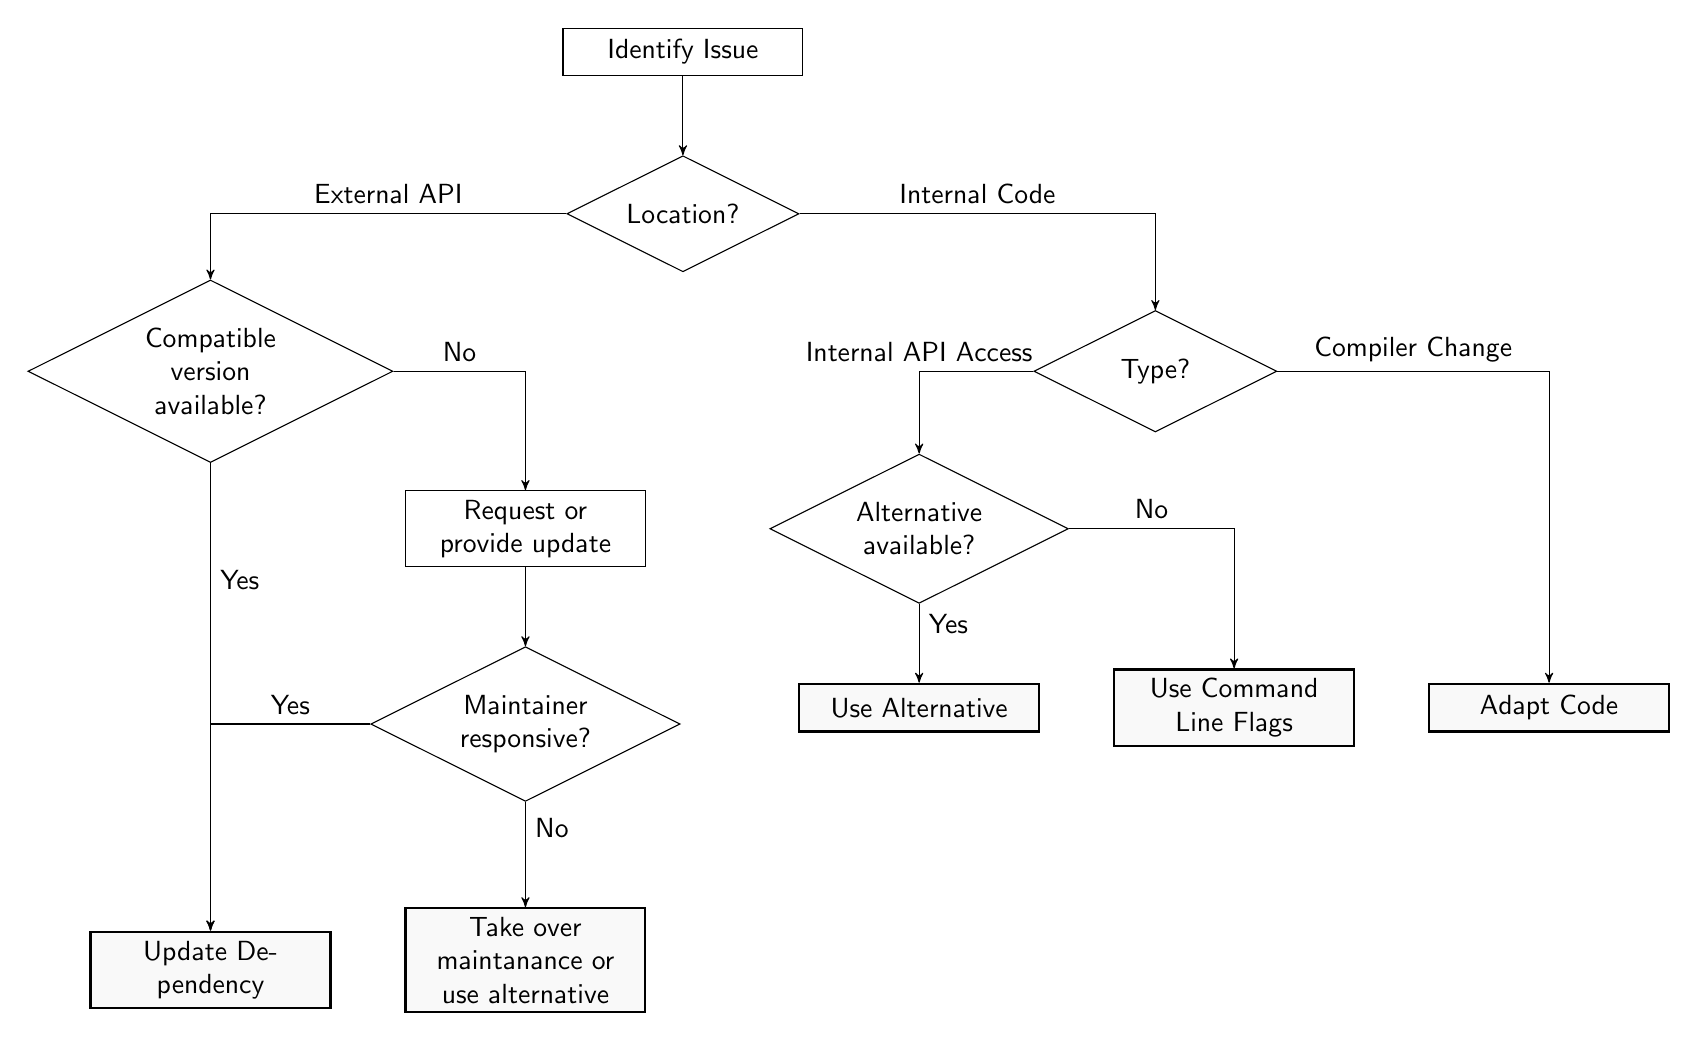
\begin{tikzpicture}[%
	every node/.style={font = \sffamily},
	>=stealth',              % Nice arrows; your taste may be different
	start chain=going below,    % General flow is top-to-bottom
	node distance=10mm and 60mm, % Global setup of box spacing
	every join/.style={norm},   % Default linetype for connecting boxes
	]
	% ------------------------------------------------- 
	% A few box styles 
	% <on chain> *and* <on grid> reduce the need for manual relative
	% positioning of nodes
	\tikzset{
		base/.style={draw, on chain, on grid, align=center, minimum height=4ex},
		proc/.style={base, rectangle, text width=8em},
		test/.style={base, diamond, aspect=2, text width=5em},
		term/.style={proc, rounded corners},
		% coord node style is used for placing corners of connecting lines
		coord/.style={coordinate, on chain, on grid, node distance=6mm and 25mm},
		% nmark node style is used for coordinate debugging marks
		nmark/.style={draw, cyan, circle, font={\sffamily\bfseries}},
		% -------------------------------------------------
		% Connector line styles for different parts of the diagram
		norm/.style={->, draw},
		free/.style={->, draw},
		cong/.style={->, draw},
		it/.style={font={\small\itshape}},
		final/.style={thick, fill=gray!5}
	}

	\node[proc] 		(p1) {Identify Issue};
	\node[test, join]	(t1) {Location?};
	
	\node[test, below left = 2cm and 6cm of t1] (t2) {Compatible version available?};
	\node[proc, below right = 2cm and 4cm of t2] (p2) {Request or provide update};
	\node[test, join]	(t3) {Maintainer responsive?};
	\node[proc, final, below = 3cm of t3] (p4) {Take over maintanance or use alternative};
	\node[proc, final, yshift=2em] at (t2 |- p4.north) (p3) {Update Dependency};
	
	\node[test, below right = 2cm and 6cm of t1] (t4) {Type?};
	\node[test, below left = 2cm and 3cm of t4] (t5) {Alternative available?};
	\node[proc, final] (p5) {Use Alternative};
	\node[proc, right = 4cm of p5, final] (p6) {Use Command Line Flags};
	\node[proc, right = 4cm of p6, final] (p7) {Adapt Code};
 	
	\draw[->] (t1) -| node[above, near start] {External API} (t2);
	\draw[->] (t2) -| node[above, near start] {No} (p2);
	\draw[->] (t2) -- node[near start, right] {Yes} (p3);
	\draw[->] (t3) -| node[above, near start] {Yes} (p3);
	\draw[->] (t3) -- node[near start, right] {No} (p4);
	\draw[->] (t1) -| node[above, near start] {Internal Code} (t4);
	\draw[->] (t4) -| node[above] {Internal API Access} (t5);
	\draw[->] (t5) -- node[near start, right] {Yes} (p5);
	\draw[->] (t5) -| node[above, near start] {No} (p6);
	\draw[->] (t4) -| node[above, near start] {Compiler Change} (p7);

	\end{tikzpicture}
	% =================================================
\end{document}